\documentclass{beamer}

\usefonttheme{professionalfonts} % using non standard fonts for beamer
\usefonttheme{serif} % default family is serif

%\usepackage{hyperref}

%\usepackage{minted}

\usepackage{animate}

\usepackage{graphicx}

\def\Put(#1,#2)#3{\leavevmode\makebox(0,0){\put(#1,#2){#3}}}

\usepackage{color}

\usepackage{tikz}

\usepackage{amssymb}

\usepackage{enumerate}


\newcommand\blfootnote[1]{%

  \begingroup

  \renewcommand\thefootnote{}\footnote{#1}%

  \addtocounter{footnote}{-1}%

  \endgroup

}

\makeatletter

%%%%%%%%%%%%%%%%%%%%%%%%%%%%%% Textclass specific LaTeX commands.

 % this default might be overridden by plain title style

 \newcommand\makebeamertitle{\frame{\maketitle}}%

 % (ERT) argument for the TOC

 \AtBeginDocument{%

   \let\origtableofcontents=\tableofcontents

   \def\tableofcontents{\@ifnextchar[{\origtableofcontents}{\gobbletableofcontents}}

   \def\gobbletableofcontents#1{\origtableofcontents}

 }

%%%%%%%%%%%%%%%%%%%%%%%%%%%%%% User specified LaTeX commands.

\usetheme{Malmoe}

% or ...

\useoutertheme{infolines}

\addtobeamertemplate{headline}{}{\vskip2pt}



\setbeamercovered{transparent}

% or whatever (possibly just delete it)

\makeatother

\begin{document}
\title[DDCEL report]{A Scalable DCEL implementation}
\author[AC]{Andres Calderon}
\institute[Spring'20]{University of California, Riverside}
\makebeamertitle
\newif\iflattersubsect

% \AtBeginSection[] {
%   \begin{frame}<beamer>
%     \frametitle{Outline} 
%     \tableofcontents[currentsection]  
%   \end{frame}
%   \lattersubsectfalse
% }

\AtBeginSubsection[] {
  \begin{frame}<beamer>
    \frametitle{Outline} 
    \tableofcontents[currentsubsection]  
  \end{frame}
}

\section*{Experiments}

%% Performance using small dataset...
\subsection{Compared to sequential tool}

\begin{frame}{Compared to sequential tool}
    \begin{itemize}
        \item Using California Census Dataset.
        \item Inputs: the census-track administrative levels for California in 2000 and 2010.
        \item Output: the merged DCEL for both inputs.
        \item Measuring time of construction for the final merged DCEL (including the DCELs for both layers and the merge).
        \item Compare the proposal (SDCEL) using different values of maximum number per partition and the sequential alternative (CGAL).
    \end{itemize}
\end{frame}

\begin{frame}{Compared to sequential tool}{General}
    \centering 
    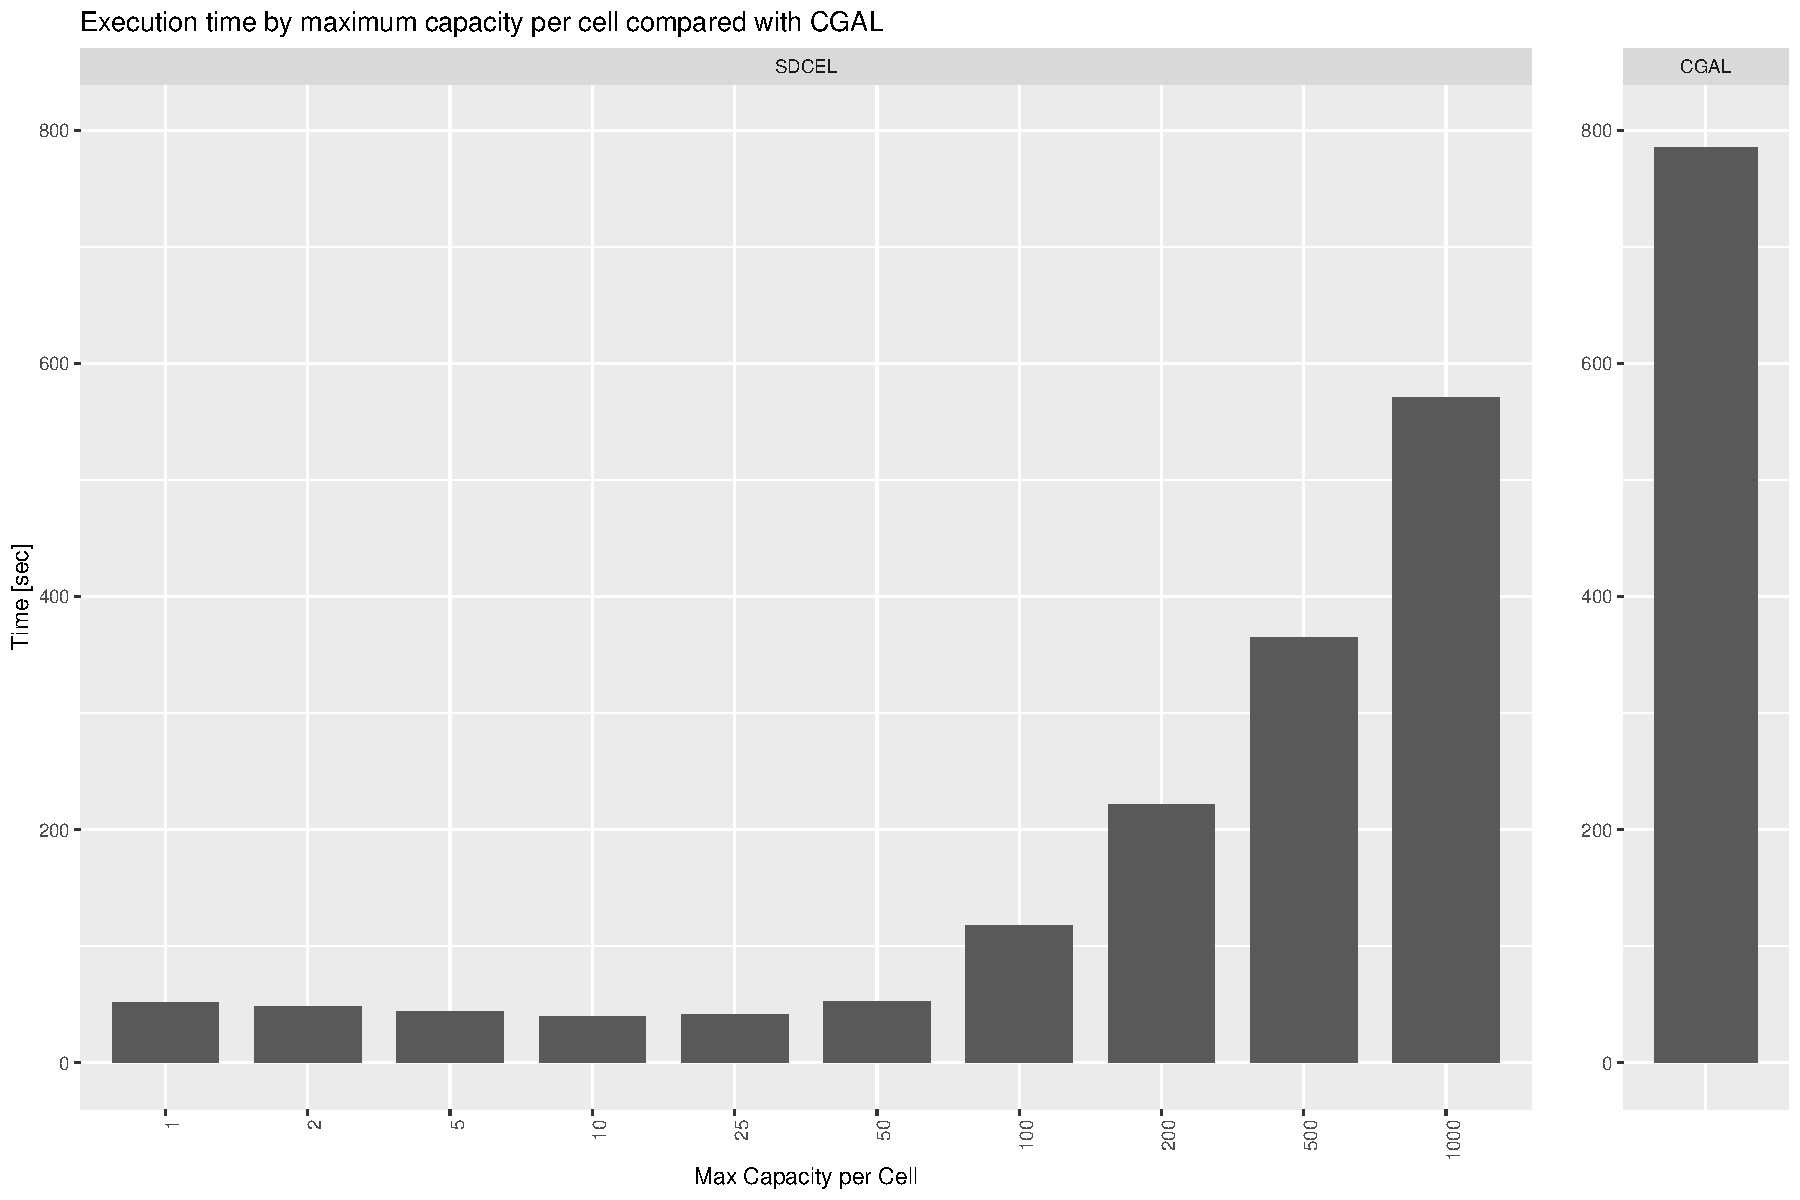
\includegraphics[width=0.9\textwidth]{figures/ca.pdf}
\end{frame}

\begin{frame}{Compared to sequential tool}{Focus on}
    \centering 
    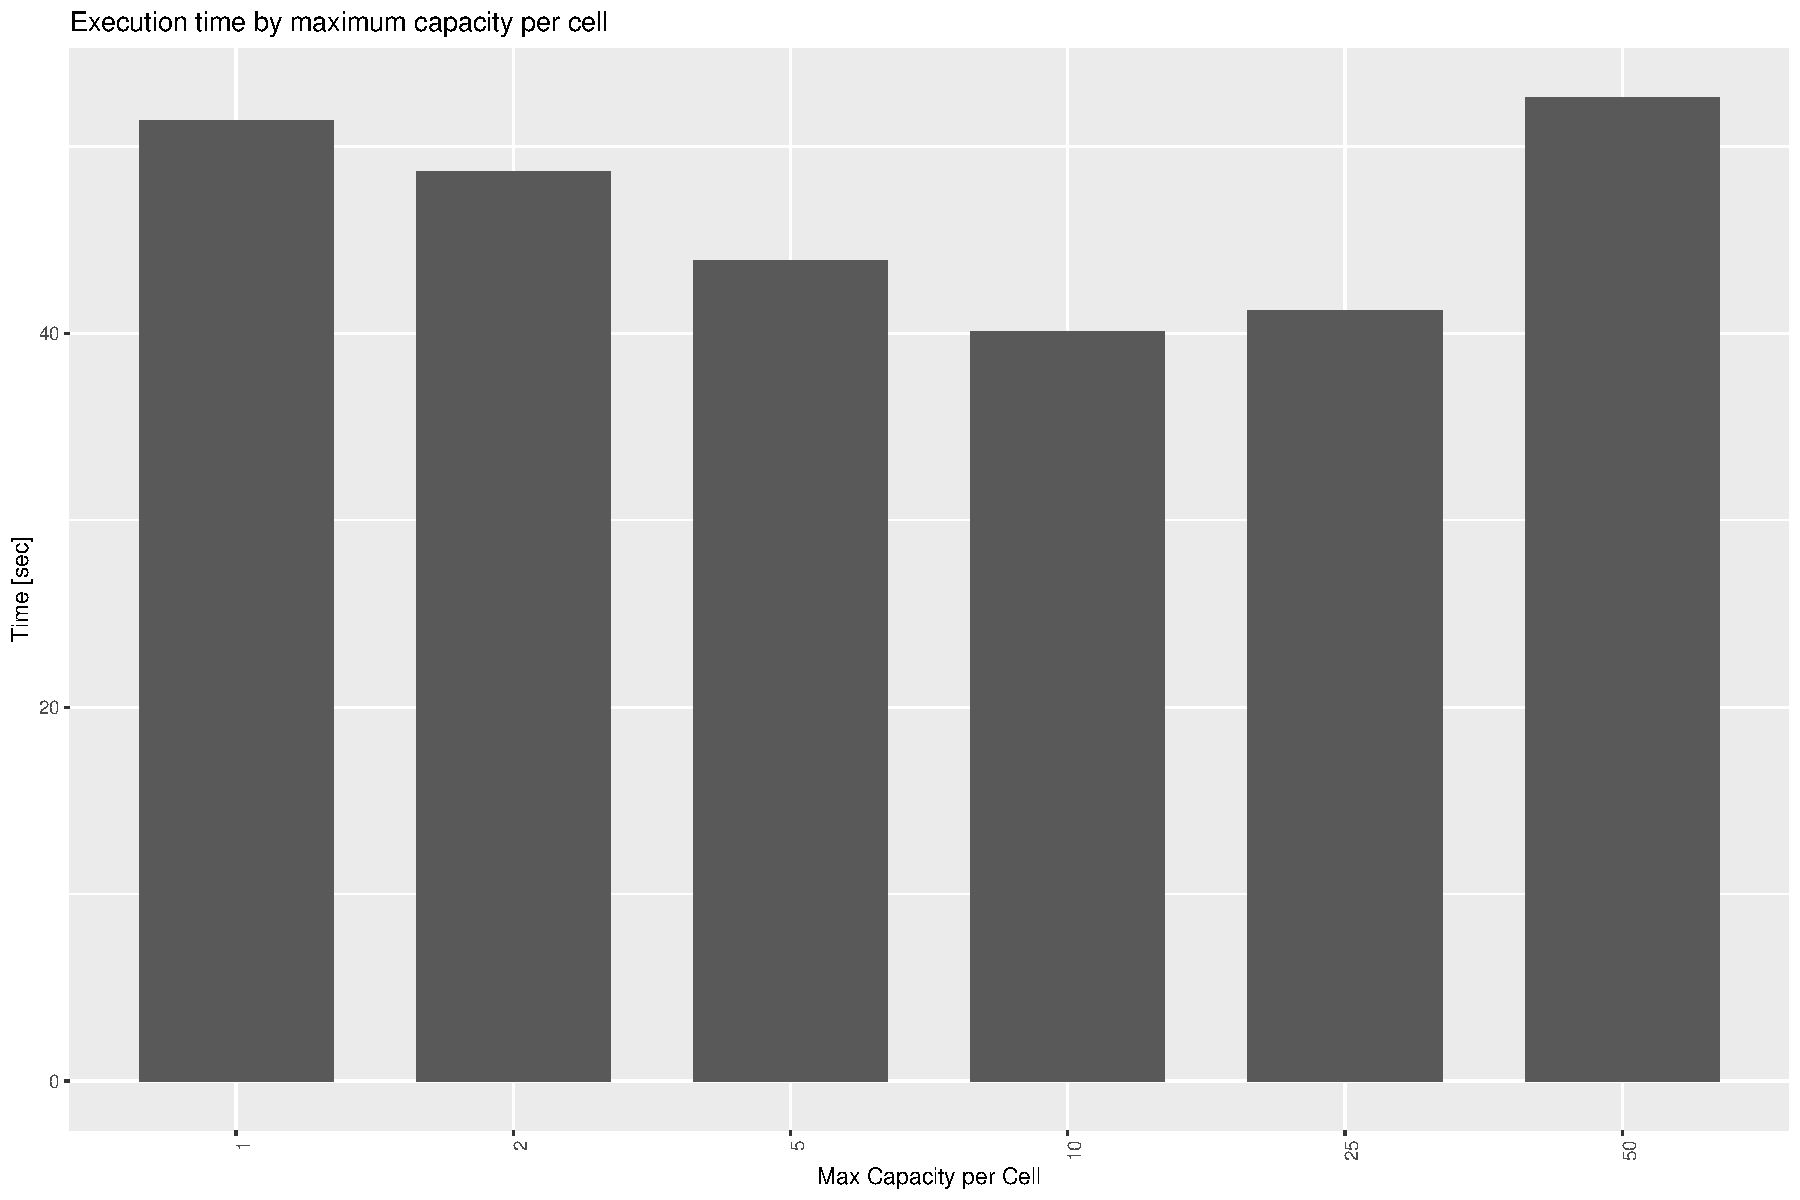
\includegraphics[width=0.9\textwidth]{figures/ca_sample.pdf}
\end{frame}

%% Performance using large dataset...
\subsection{Compared to 1-core execution}

\begin{frame}{Compared to 1-core execution}
    \begin{itemize}
        \item Using GADM Dataset.
        \item Inputs: Administrative levels for the whole world.  Level 0 (Countries) and Level 1 (States) disaggregated by individual polygons.
        \item Output: the merged DCEL for both inputs.
        \item Measuring time of construction for the final merged DCEL (including the DCELs for both layers and the merge).
        \item Compare SDCEL using different number of partitions and SDCEL running on just 1 core.
    \end{itemize}
\end{frame}
\begin{frame}{Compared to 1-core execution}{General}
    \centering 
    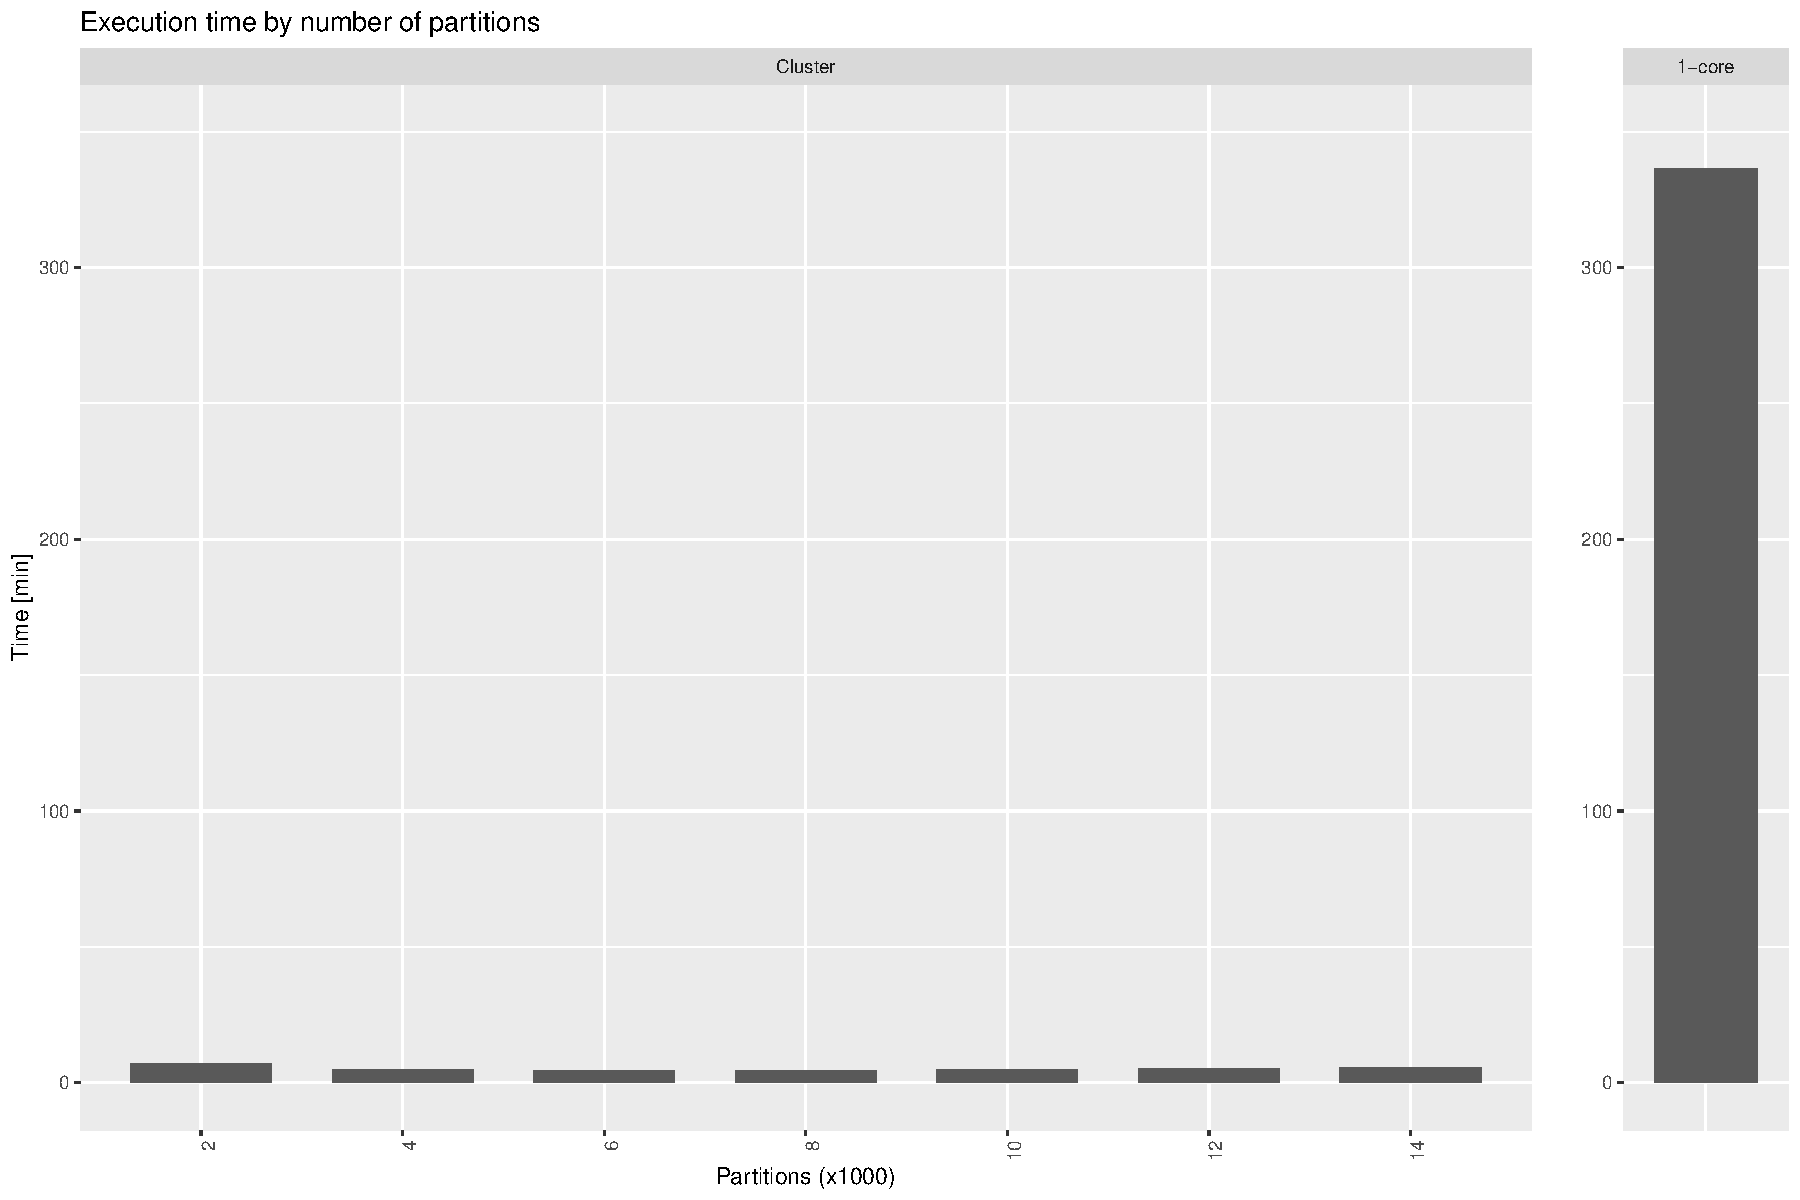
\includegraphics[width=0.9\textwidth]{figures/gadm.pdf}
\end{frame}
\begin{frame}{Compared to 1-core execution}{Focus on}
    \centering 
    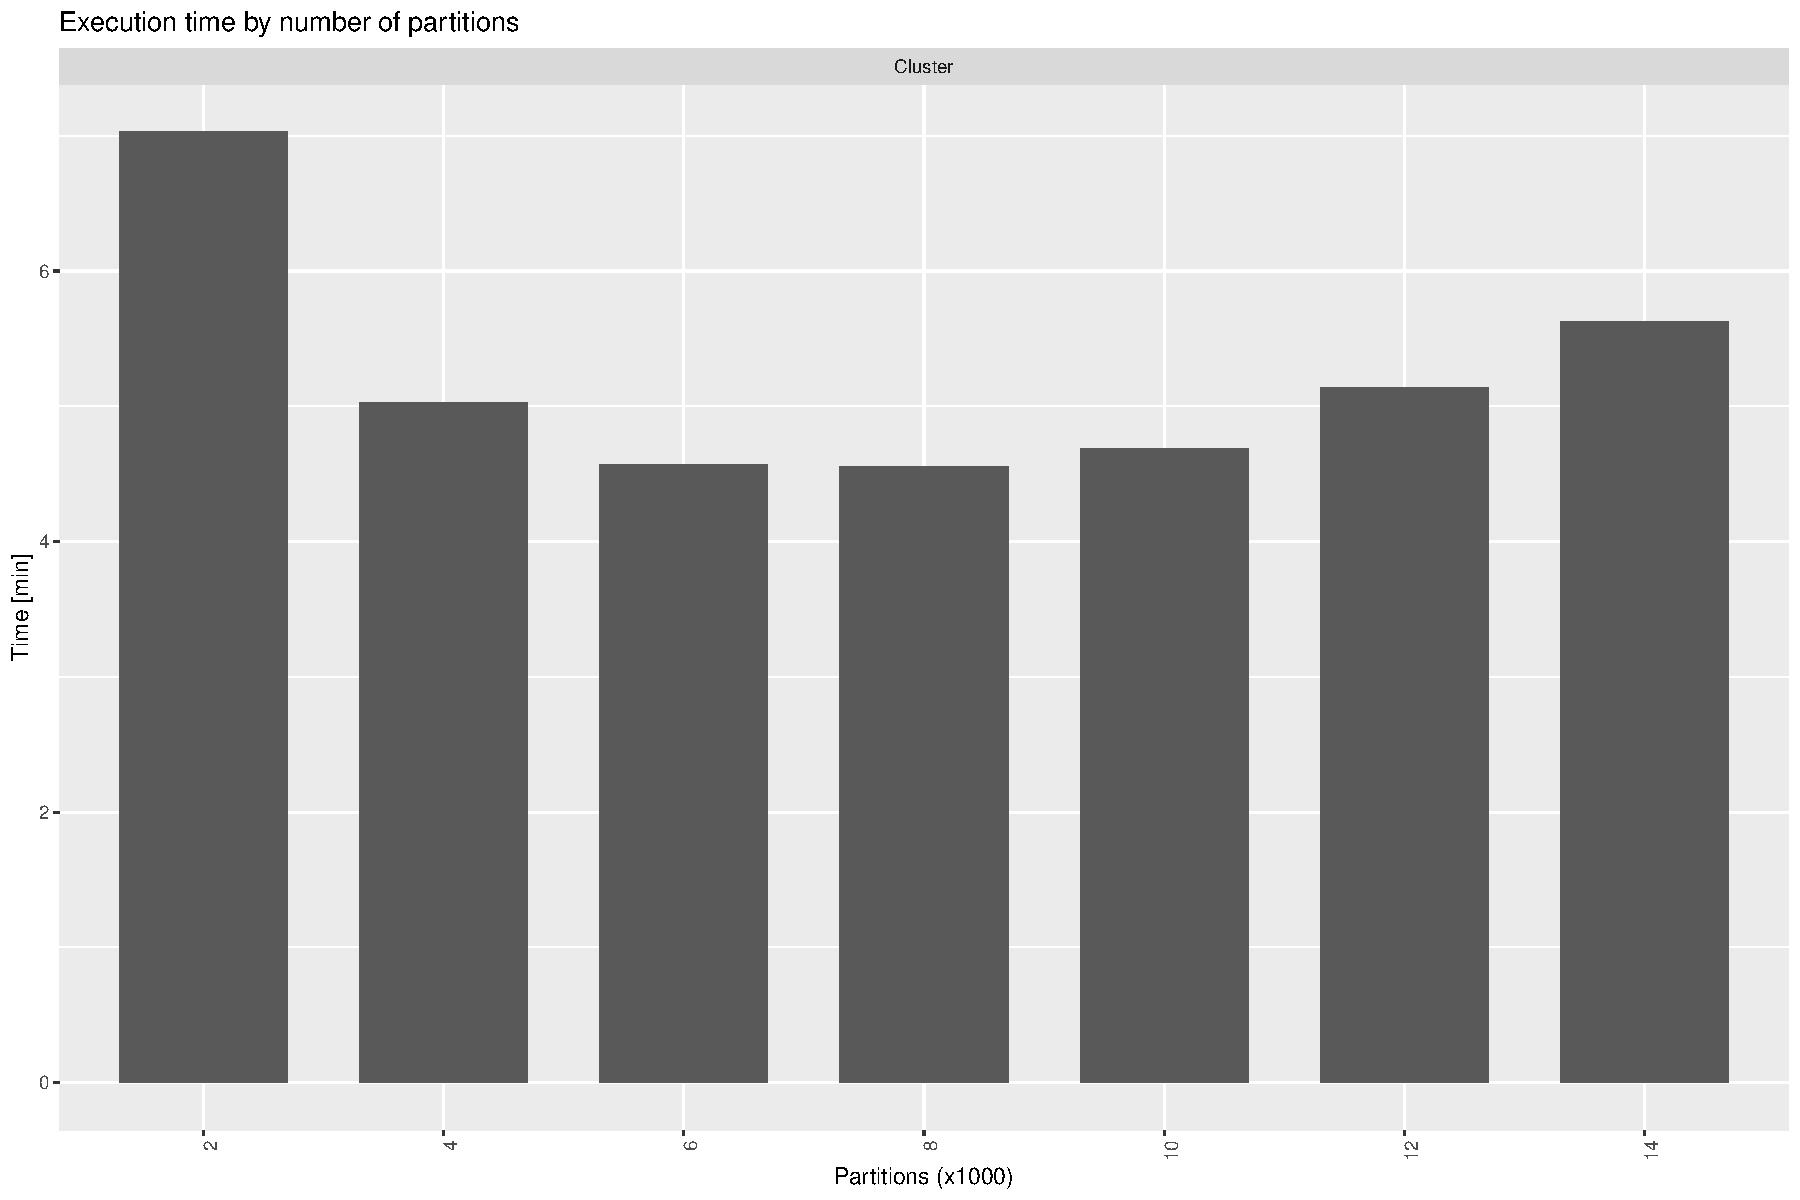
\includegraphics[width=0.9\textwidth]{figures/gadm_sample.pdf}
\end{frame}

%% Speed up analysis...
\subsection{Speed up Analysis}

\begin{frame}{Speed up Analysis}
    \begin{itemize}
        \item Using GADM Dataset.
        \item Inputs: Administrative levels for the whole world.  Level 0 (Countries) and Level 1 (States) disaggregated by individual polygons.
        \item Output: the merged DCEL for both inputs.
        \item Measuring time of construction for the final merged DCEL.
        \item Compare SDCEL using different number of nodes (each node with 9 cores).
    \end{itemize}
\end{frame}
\begin{frame}{Speed up Analysis}
    \centering 
    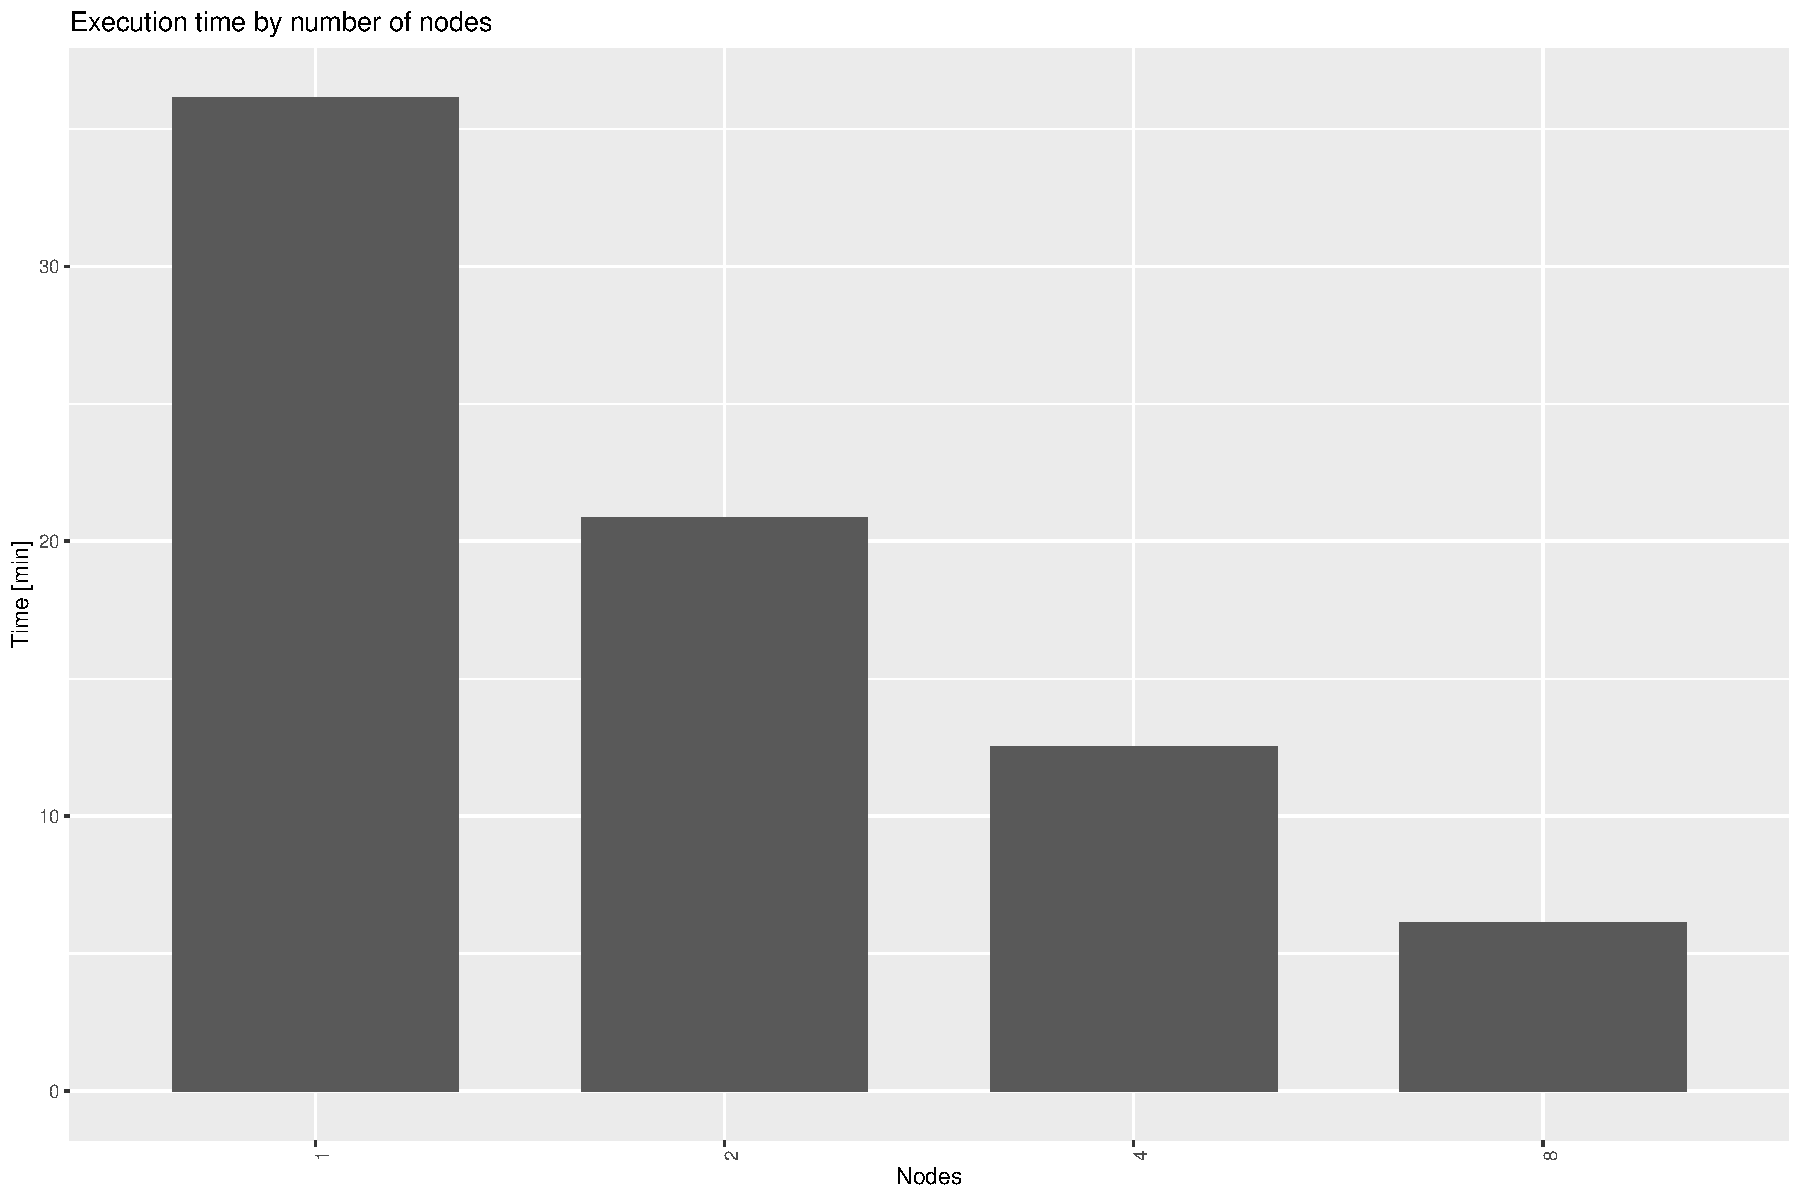
\includegraphics[width=0.9\textwidth]{figures/speedup.pdf}
\end{frame}

%% Scale up analysis...
\subsection{Scale up Analysis}

\begin{frame}{Scale up Analysis}
    \begin{itemize}
        \item Using GADM Dataset.
        \item Inputs: 4 sections of the previous GADM dataset spatially dividing its extension in approximate the same number of polygons and edges. 
        \item Output: the merged DCEL for both inputs to each section.
        \item Measuring time of construction for the final merged DCEL.
        \item Compare SDCEL increasing the size of the inputs (1 section, 2 sections, 3 section and 4 sections) and also increasing number of available nodes.
    \end{itemize}
\end{frame}
\begin{frame}{Scale up Analysis}
    \centering 
    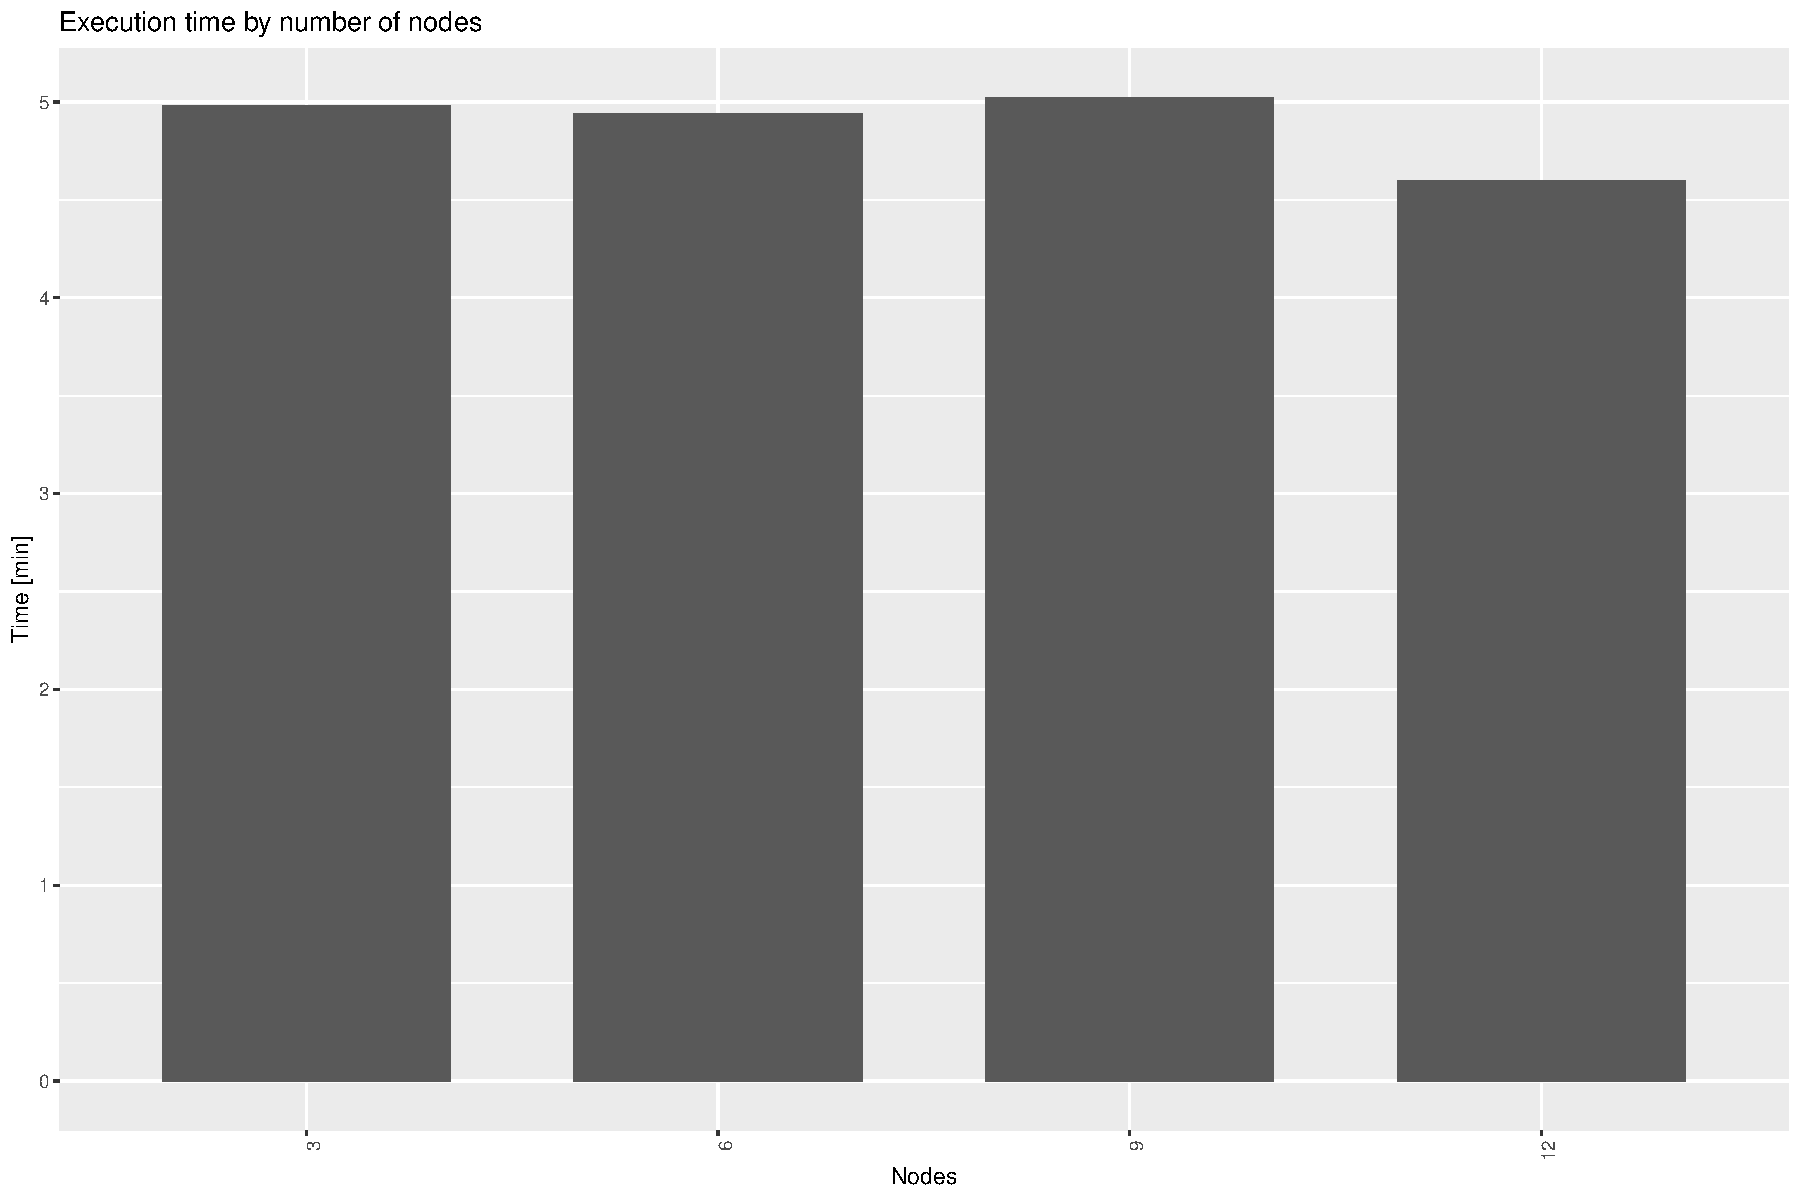
\includegraphics[width=0.9\textwidth]{figures/scaleup.pdf}
\end{frame}

\end{document}
